%%%%%%%%%%%%%%%%%%%%%%%%%%%%%%%%%%%%%%%%%%%%%%%%%%%%%%%%%%%%%%%%%%%%%
%%                                                                 %%
%% Please do not use \input{...} to include other tex files.       %%
%% Submit your LaTeX manuscript as one .tex document.              %%
%%                                                                 %%
%% All additional figures and files should be attached             %%
%% separately and not embedded in the \TeX\ document itself.       %%
%%                                                                 %%
%%%%%%%%%%%%%%%%%%%%%%%%%%%%%%%%%%%%%%%%%%%%%%%%%%%%%%%%%%%%%%%%%%%%%

%%\documentclass[referee,sn-basic]{sn-jnl}% referee option is meant for double line spacing

%%=======================================================%%
%% to print line numbers in the margin use lineno option %%
%%=======================================================%%

%%\documentclass[lineno,sn-basic]{sn-jnl}% Basic Springer Nature Reference Style/Chemistry Reference Style

%%======================================================%%
%% to compile with pdflatex/xelatex use pdflatex option %%
%%======================================================%%

%%\documentclass[pdflatex,sn-basic]{sn-jnl}% Basic Springer Nature Reference Style/Chemistry Reference Style

%%\documentclass[sn-basic]{sn-jnl}% Basic Springer Nature Reference Style/Chemistry Reference Style
\documentclass[pdflatex,sn-mathphys]{sn-jnl}% Math and Physical Sciences Reference Style
%%\documentclass[sn-aps]{sn-jnl}% American Physical Society (APS) Reference Style
%%\documentclass[sn-vancouver]{sn-jnl}% Vancouver Reference Style
%%\documentclass[sn-apa]{sn-jnl}% APA Reference Style
%%\documentclass[sn-chicago]{sn-jnl}% Chicago-based Humanities Reference Style
%%\documentclass[sn-standardnature]{sn-jnl}% Standard Nature Portfolio Reference Style
%%\documentclass[default]{sn-jnl}% Default
%%\documentclass[default,iicol]{sn-jnl}% Default with double column layout

%%%% Standard Packages
%%<additional latex packages if required can be included here>
%%%%

%%%%%=============================================================================%%%%
%%%%  Remarks: This template is provided to aid authors with the preparation
%%%%  of original research articles intended for submission to journals published 
%%%%  by Springer Nature. The guidance has been prepared in partnership with 
%%%%  production teams to conform to Springer Nature technical requirements. 
%%%%  Editorial and presentation requirements differ among journal portfolios and 
%%%%  research disciplines. You may find sections in this template are irrelevant 
%%%%  to your work and are empowered to omit any such section if allowed by the 
%%%%  journal you intend to submit to. The submission guidelines and policies 
%%%%  of the journal take precedence. A detailed User Manual is available in the 
%%%%  template package for technical guidance.
%%%%%=============================================================================%%%%

\jyear{2021}%

%% as per the requirement new theorem styles can be included as shown below
\theoremstyle{thmstyleone}%
\newtheorem{theorem}{Theorem}%  meant for continuous numbers
%%\newtheorem{theorem}{Theorem}[section]% meant for sectionwise numbers
%% optional argument [theorem] produces theorem numbering sequence instead of independent numbers for Proposition
\newtheorem{proposition}[theorem]{Proposition}% 
%%\newtheorem{proposition}{Proposition}% to get separate numbers for theorem and proposition etc.

\theoremstyle{thmstyletwo}%
\newtheorem{example}{Example}%
\newtheorem{remark}{Remark}%

\theoremstyle{thmstylethree}%
\newtheorem{definition}{Definition}%

\raggedbottom
%%\unnumbered% uncomment this for unnumbered level heads

\begin{document}

\title[An Effectively Complexity-reduced Language Model for Text Classification]{DistilBERT: An Effectively Complexity-reduced Language Model for Text Classification}

%%=============================================================%%
%% Prefix	-> \pfx{Dr}
%% GivenName	-> \fnm{Joergen W.}
%% Particle	-> \spfx{van der} -> surname prefix
%% FamilyName	-> \sur{Ploeg}
%% Suffix	-> \sfx{IV}
%% NatureName	-> \tanm{Poet Laureate} -> Title after name
%% Degrees	-> \dgr{MSc, PhD}
%% \author*[1,2]{\pfx{Dr} \fnm{Joergen W.} \spfx{van der} \sur{Ploeg} \sfx{IV} \tanm{Poet Laureate} 
%%                 \dgr{MSc, PhD}}\email{iauthor@gmail.com}
%%=============================================================%%

\author*[1,3,4]{\fnm{Ngoc-Thien-An} \sur{Pham}}\email{pntan19@clc.fitus.edu.vn}

\author[2,3,4]{\fnm{Hoang-Quan} \sur{Tran}}\email{19120338@student.hcmus.edu.vn}
\equalcont{These authors contributed equally to this work.}

% \author[1,2]{\fnm{Third} \sur{Author}}\email{iiiauthor@gmail.com}
% \equalcont{These authors contributed equally to this work.}

\affil*[1]{\orgdiv{Department of Computer Science}}

\affil[2]{\orgdiv{Department of Knowledge Engineering}}

\affil[3]{\orgname{Faculty of Information Technology, University of Science}}

\affil[4]{\orgname{Vietnam National University}, \orgaddress{\city{Ho Chi Minh City}, \country{Vietnam}}}

%%==================================%%
%% sample for unstructured abstract %%
%%==================================%%

\abstract{Text classification has been a fundamental task since the early days of Natural Language Processing. Recently, the invention of large language models such as BERT, RoBERTa, XLM, and others has started a revolution in Natural Language Processing, specifically in Text Classification and text-related tasks. However, these models require an enormous contextual dataset, a high-cost training environment, and a long training time to achieve a notable result. This paper presents a novel approach to Text Classification using a lighter, cheaper, faster version of BERT called DistilBERT. By fine-tuning DistilBERT for the Text Classification task, we achieved a state-of-the-art result of 97,40\%, 97,61\%, 97,74\%, and 97,64\% in accuracy, macro precision, macro recall, and macro F1 respectively. With these evaluation metrics, our model outperformed the current state-of-the-art language model and other approaches in the text classification task.}

%%================================%%
%% Sample for structured abstract %%
%%================================%%

% \abstract{\textbf{Purpose:} The abstract serves both as a general introduction to the topic and as a brief, non-technical summary of the main results and their implications. The abstract must not include subheadings (unless expressly permitted in the journal's Instructions to Authors), equations or citations. As a guide the abstract should not exceed 200 words. Most journals do not set a hard limit however authors are advised to check the author instructions for the journal they are submitting to.
% 
% \textbf{Methods:} The abstract serves both as a general introduction to the topic and as a brief, non-technical summary of the main results and their implications. The abstract must not include subheadings (unless expressly permitted in the journal's Instructions to Authors), equations or citations. As a guide the abstract should not exceed 200 words. Most journals do not set a hard limit however authors are advised to check the author instructions for the journal they are submitting to.
% 
% \textbf{Results:} The abstract serves both as a general introduction to the topic and as a brief, non-technical summary of the main results and their implications. The abstract must not include subheadings (unless expressly permitted in the journal's Instructions to Authors), equations or citations. As a guide the abstract should not exceed 200 words. Most journals do not set a hard limit however authors are advised to check the author instructions for the journal they are submitting to.
% 
% \textbf{Conclusion:} The abstract serves both as a general introduction to the topic and as a brief, non-technical summary of the main results and their implications. The abstract must not include subheadings (unless expressly permitted in the journal's Instructions to Authors), equations or citations. As a guide the abstract should not exceed 200 words. Most journals do not set a hard limit however authors are advised to check the author instructions for the journal they are submitting to.}

\keywords{Text classification, Natural language processing, Deep learning, Knowledge distillation, Pretrained language models}

%%\pacs[JEL Classification]{D8, H51}

%%\pacs[MSC Classification]{35A01, 65L10, 65L12, 65L20, 65L70}

\maketitle

\section{Introduction}\label{introduction}
sede vacante

\section{Related works}\label{relatedworks}
\subsection{Shallow machine-learning models}

Shallow machine-learning approaches are traditional machine-learning techniques that involve the extraction of hand-crafted features from the text. Early approaches to the Text Classification problem using rule-based systems where an expert suggests a rule for classifying text, based on the semantics and pragmatics of the data. Later on, several methods including Naive Bayes\cite{Xu2017}, Decision Trees\cite{Safavian1991}, Logistic Regression\cite{Genkin2007} and Support Vector Machine (SVM)\cite{boser1992, cortesvapnik1995} were proposed with the concept of using the probability of tokens to predict if a document belongs to a specific class. 

These approaches are easy to implement and perform best with a small amount of data. Besides advantages, shallow models have some disadvantages by requiring a feature engineering step to be effective. Additionally, shallow learning method's output are depending on the probability of each token, which is not capturing the general semantics of a complex document.

\subsection{Deep learning models}
\subsubsection{Convolutional Neural Network (CNN)}
Unlike shallow methods, deep learning methods automatically learn features from the data. Kim et al (2014) introduced a Convolutional Neural Network (CNN) approach, which uses a simple CNN with one layer of convolution on top of pre-trained word vectors\cite{Kim2014}. Using an unsupervised learning model, an input word is converted into a word representation vector in a contextual space and then stacked to form a sentence-representation matrix. The representation matrix then goes through a number of convolutional, pooling and fully connected layers with the final output being the probability distribution over labels.

The architecture described in the work of Kim et al. (2014) is presented in Figure~\ref{fig:kim2014}

\begin{figure}[htp]
\centering
\resizebox{\textwidth}{!}{
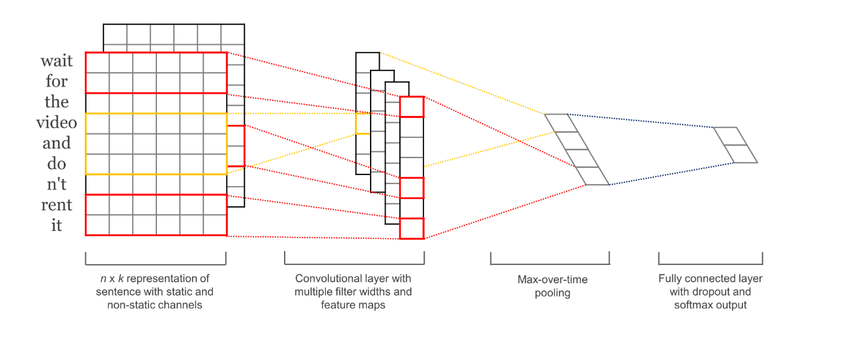
\includegraphics{cnn-classification.png}
}
\caption{The CNN for text classification architecture described in the work of Kim et al. (2014)\cite{Kim2014}}
\label{fig:kim2014}
\end{figure}

\subsubsection{Sequence-to-Sequence using Recurrent Neural Network (RNN)}
Cho et al. (2014)\cite{Cho2014} and Sutskever et al. (2014)\cite{Sutskever2014} proposed an architecture named Sequence-to-Sequence (Seq2Seq) to solve the Machine Translation problem. Given an input sentence $s$ defined as a sequence of tokens $s_1, s_2, .., s_n$. The input sequence is fed into the Encoder, which is designed as a Recurrent Neural Network (RNN) to extract the context vector $h_s$ as the sentence-representation vector. The vector $h_s$ is then fed into the Decoder as the initial hidden state to generate the output sequence $s’_1, s’_2, .., s’_n$ as the translation of the sentence $s$ in a second language. An illustration of the proposed approach of Cho et al. (2014) and Sutskever et al. (2014) is presented in Figure~\ref{fig:seq2seq}

\begin{figure}[htp]
\centering
\resizebox{\textwidth}{!}{
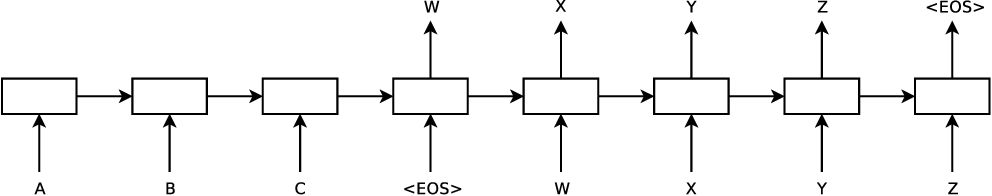
\includegraphics{seq2seq.png}
}
\caption{The Sequence-to-Sequence architecture proposed by Cho et al. (2014)\cite{Cho2014}}
\label{fig:seq2seq}
\end{figure}

Assuming the output vector $h_s$ of Encoder is the representation vector of sentence $s$, we can feed $h_s$ through a fully connected layer to get the probability of each label. A visualization of the Sequence-to-Sequence architecture for text classification can be described in Figure~\ref{fig:seq2seq-classification}

\begin{figure}[htp]
\centering
\resizebox{\textwidth}{!}{
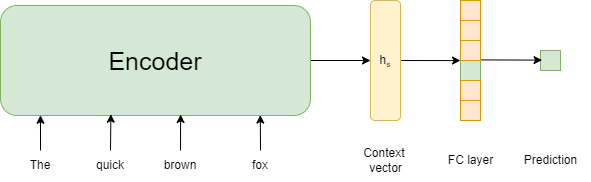
\includegraphics{seq2seq-classification.png}
}
\caption{A Sequence-to-Sequence architecture for text classification}
\label{fig:seq2seq-classification}
\end{figure}

\subsubsection{Ensemble between CNN and LSTM}


\subsubsection{BERT}

\subsubsection{XLNet}

These models have shown state-of-the-art performance on many text classification tasks but require significantly more computational resources and data to train effectively. However, these models are highly scalable, making them suitable for processing large amounts of text data.


\section{Proposed method}\label{proposedmethod}
sede vacante

\section{Experiments}\label{experiments}
\subsection{Baselines}
sede vacante

\subsection{Dataset}
Experiments were conducted on the TREC-6 dataset including 6000 sentences divided into training/testing sets with 5500 for training and 500 for testing. We use the TREC-6 training set for training and finetuning while evaluations were made on the testing set. The dataset’s statistics are briefly described in Table~\ref{tab:trec-6-insight}

\begin{table}[htp]
\centering
\caption{Insight of the TREC-6 dataset} \label{tab:trec-6-insight}
\resizebox{\textwidth}{!}{
\begin{tabular}{llllll}
\hline
\textbf{Training} & \textbf{Testing} & \textbf{Coarse labels} & \textbf{Fine class labels} & \textbf{Avg. length} & \textbf{Vocab. size} \\ \hline
5500              & 500              & 6                      & 50                         & 10                   & 8700                 \\ \hline
\end{tabular}
}
\end{table}

\subsection{Hyperparameters settings}
sede vacante

\subsection{Analysis}
sede vacante

\subsection{Discussions}
sede vacante

\section{Conclusion and Future works}\label{conclusionandfutureworks}
sede vacante

%%===========================================================================================%%
%% If you are submitting to one of the Nature Portfolio journals, using the eJP submission   %%
%% system, please include the references within the manuscript file itself. You may do this  %%
%% by copying the reference list from your .bbl file, paste it into the main manuscript .tex %%
%% file, and delete the associated \verb+\bibliography+ commands.                            %%
%%===========================================================================================%%

\bibliography{sn-bibliography}% common bib file
%% if required, the content of .bbl file can be included here once bbl is generated
%%\input sn-article.bbl

%% Default %%
%%\input sn-sample-bib.tex%

\end{document}
